\chapter{Geheugenarchitectuur}
\label{architecture}
De afzonderlijke geheugencellen zullen samengebracht worden in een geheel.
Dit hoofdstuk bespreekt de algemene structuur alsook de vrijheidsgraden die in hoofdstuk \ref{timing-optimization} onderzocht worden om tot een optimaal werkend systeem te komen. Ten slotte zullen ook nog de bouwblokken aangekaard worden die meer uitvoerig besproken worden in de volgende hoofdstukken. 


\section{Cel}
Zoals besproken in hoofdstuk \ref{cell} is dit het bouwblok dat het vaakst terug te vinden is in het geheugensysteem.
De cel bestaat uit een memristor en een transistor (1T1R-cel). De geheugencel heeft drie terminals: de gate van de transistor, die verbonden wordt met een wordline, de source van de transistor, die verbonden wordt met een sourceline en tenslotte de terminal van de memristor, die verbonden wordt met een bitline.
%Een cel waarvan memristor zich in een willekeurige resistieve staat bevindt is een datacel, terwijl de memristor van referentiecellen in een voorgeprogrammeerde en dus gekende resistieve staat verkeert.

\section{Branch}
In een branch worden er een bepaald aantal datacellen verbonden aan één BL en één SL. Dit aantal wordt \emph{Number of Word Lines per Branch} (NoWLpB) genoemd en is een van de vrijheidsgraden van de geheugenarchitectuur. Naast alle datacellen is er ook nog één referentiecel - dit zijn cellen waarvan de resistieve staat voorgeschreven is - verbonden aan de BL en SL van de branch.
Elke BL wordt via een pMOS-transistor (al dan niet met nog een impedantie tussenin) gekoppeld aan de voedingspanning Vdd en via een nMOS-transistor aan de grondspanning Vss. In dit werk is er enkel een nMOS-transistor die de SL verbindt met Vss.\footnote{In een volledig geheugensysteem zou de SL via een pMOS ook nog verbonden zijn met een niet onderzochte spanningsknoop Vdd\_write. De pMOS zou dan worden aangezet voor schrijfwerking.} De nMOS-transistoren aan BL en SL fungeren als schakelaars, de pMOS-transistor wordt daarenboven ook gebruikt als impedantie voor een resistieve spanningsdeling (zie hoofdstuk \ref{loadanalysis}).
Ter illustratie wordt de samenhang tussen cel en branch getoond in figuur \ref{fig:cellbranch}.

\begin{figure}
  \centering
  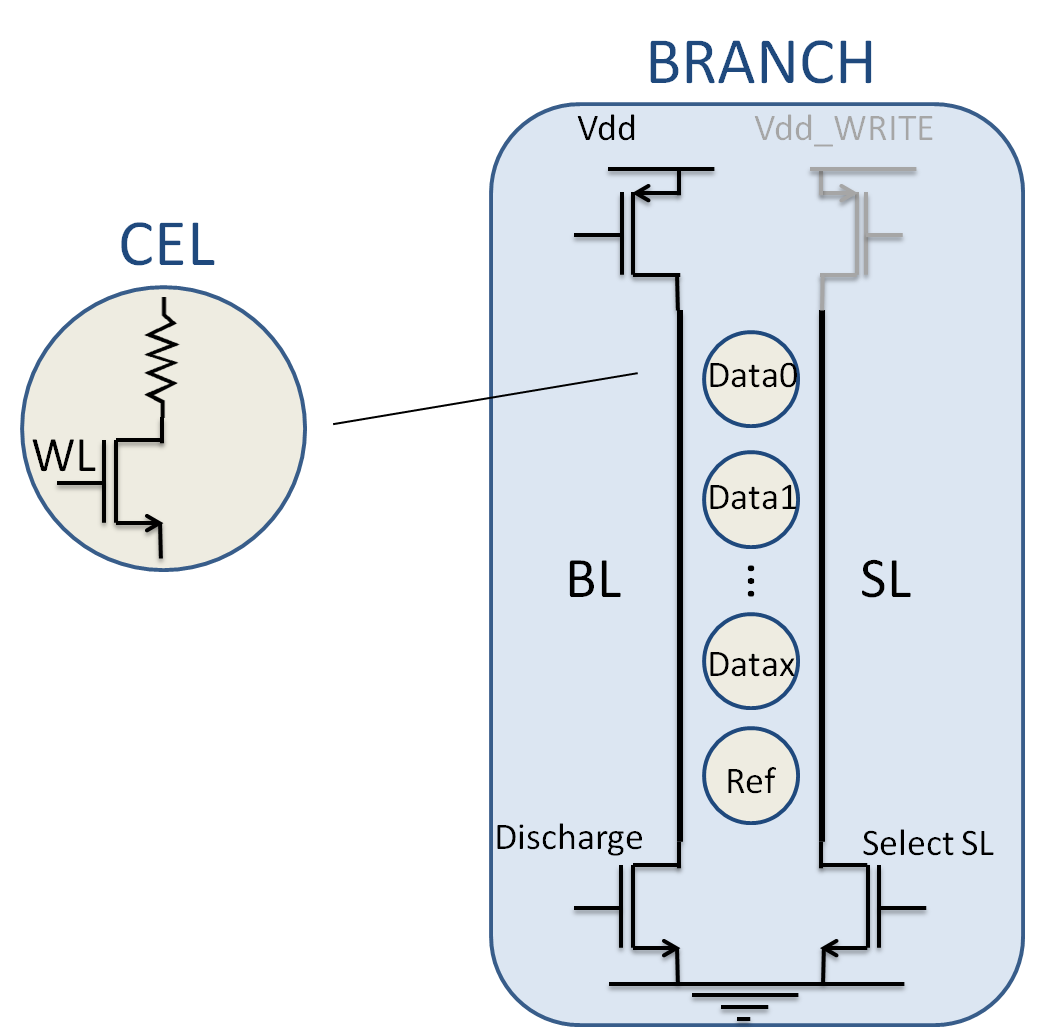
\includegraphics[scale=0.3]{../fig/hfdstk-architecture-cell-branch.png}
  \caption{Een geheugencel en een branch}
  \label{fig:cellbranch}
\end{figure}

\section{Local Block}
Verschillende BLs en SLs worden samengebracht in een local block, waarvan de vrijheidsgraad \emph{Number of BitLines per Local Block} (NoBLpLB) heet. In een LB bevinden er zich dus NoBLpLB x NoWLpB datacellen en NoBLpLB referentiecellen. Ook bevat een local block zowel BL- als WL-decoders. De afzonderlijke BLs worden via passgates verbonden tot een uitgangsknooppunt.
De structuur van een local block is geïllustreerd op figuur \ref{fig:LB}.
De uitgangen van de WL-decoder sturen de data-WLs aan [eventueel met een buffer], de uitgangen van de BL-decoder activeren een spanningsdeling op de BLs.\footnote{Indien schrijfwerking zou toegevoegd worden, zouden de uitgangen van de BL-decoder aan twee AND-poorten worden verbonden; bij leesoperatie brengt de uitgang van de ene AND-poort de resistieve deling op de BL teweeg, bij schrijfoperatie zet de uitgang van de andere AND-poort een pull-up-operatie van de BL naar Vdd\_write op.} De referentie-WL is via een extern signaal verbonden. Voor een gedetailleerdere beschrijving over hoe de decoderuitgangen gebruikt worden, zie sectie \ref{timing}.
Aangezien een LB zowel data- als referentiecellen bevat, gaat een LB twee werkingsmodes hebben: een mode waarbij er één datacel wordt aangesproken en een mode waarbij er een bepaald aantal referentiecellen in parallel wordt aangesproken.
Figuur \ref{fig:LB-details} geeft een meer gedetailleerd beeld van een LB, decoders weggelaten.

\begin{figure}
  \centering
  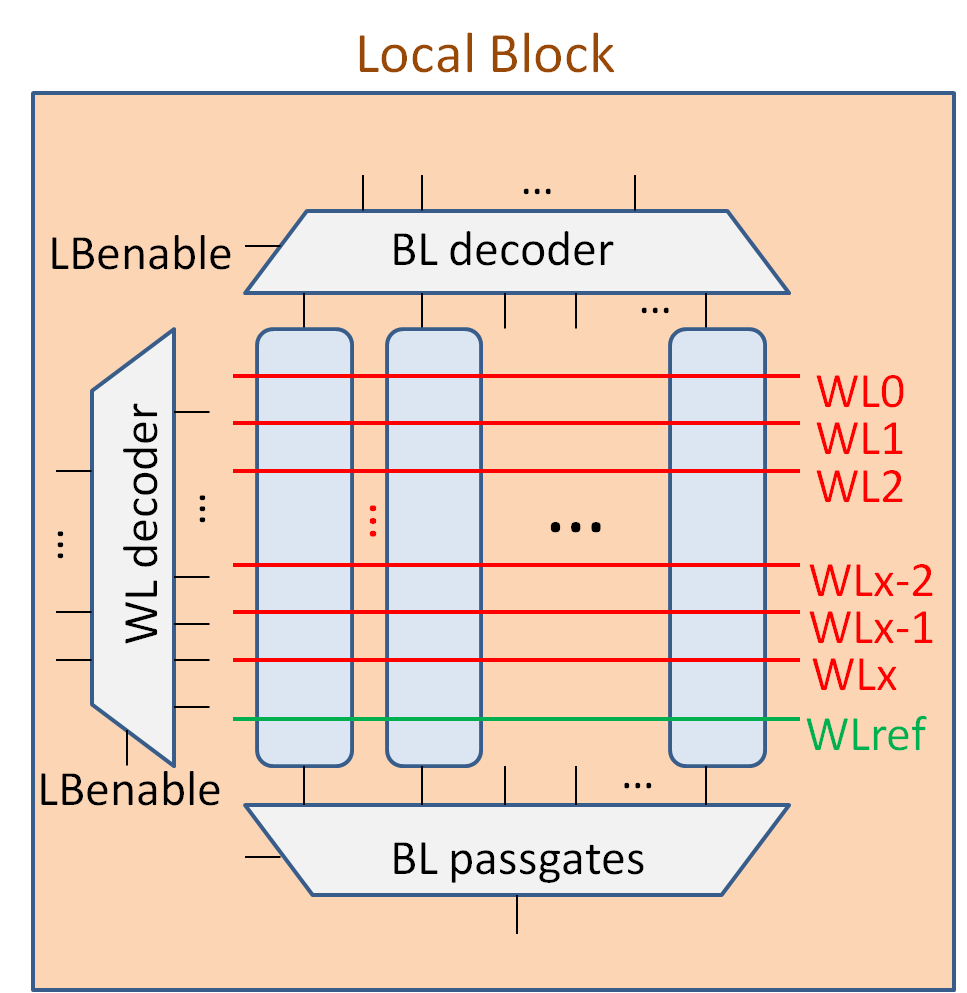
\includegraphics[scale=0.3]{../fig/hfdstk-architecture-localblock.png}
  \caption{Een Local Block}
  \label{fig:LB}
\end{figure}

\begin{figure}
  \centering
  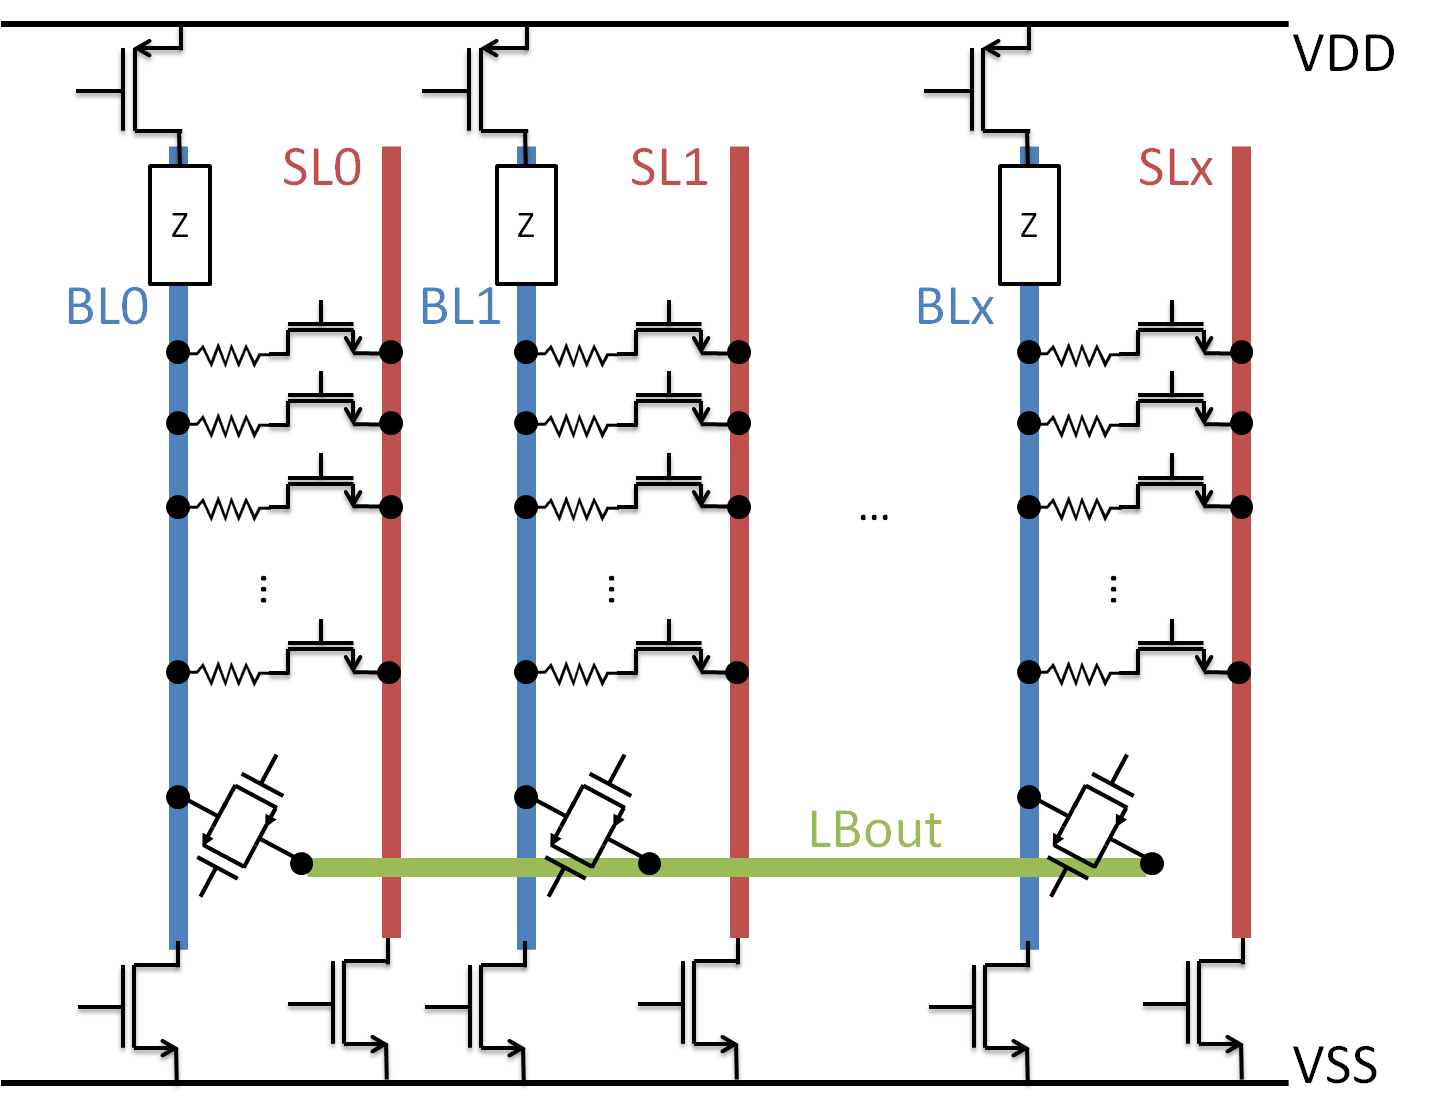
\includegraphics[scale=0.3]{../fig/hfdstk-architecture-LB-details.png}
  \caption{Een meer gedetailleerde illustratie van een LB, decoders zijn weggelaten}
  \label{fig:LB-details}
\end{figure}

\subsection{Datasignaal uitlezen}
Het datasignaal is de spanning op de BL nadat er een resistieve deling is gebeurd, waarbij er stroom vloeit door één cel. De last die hangt aan de voedingsspanning, op figuur \ref{fig:dataread} voorgesteld als een pMOS-transistor, wordt aangeschakeld, alsook de nMOS-transistoren in de cel en aan de sourceline. Er vloeit een stroom langs dit pad: I=Vdd/Rtot, en de spanning op de BL is V=IReq. Om dit datasignaal op de uitgangsknoop van het LB te krijgen, wordt de bijhorende passgate van de BL in kwestie geactiveerd.

\begin{figure}
  \centering
  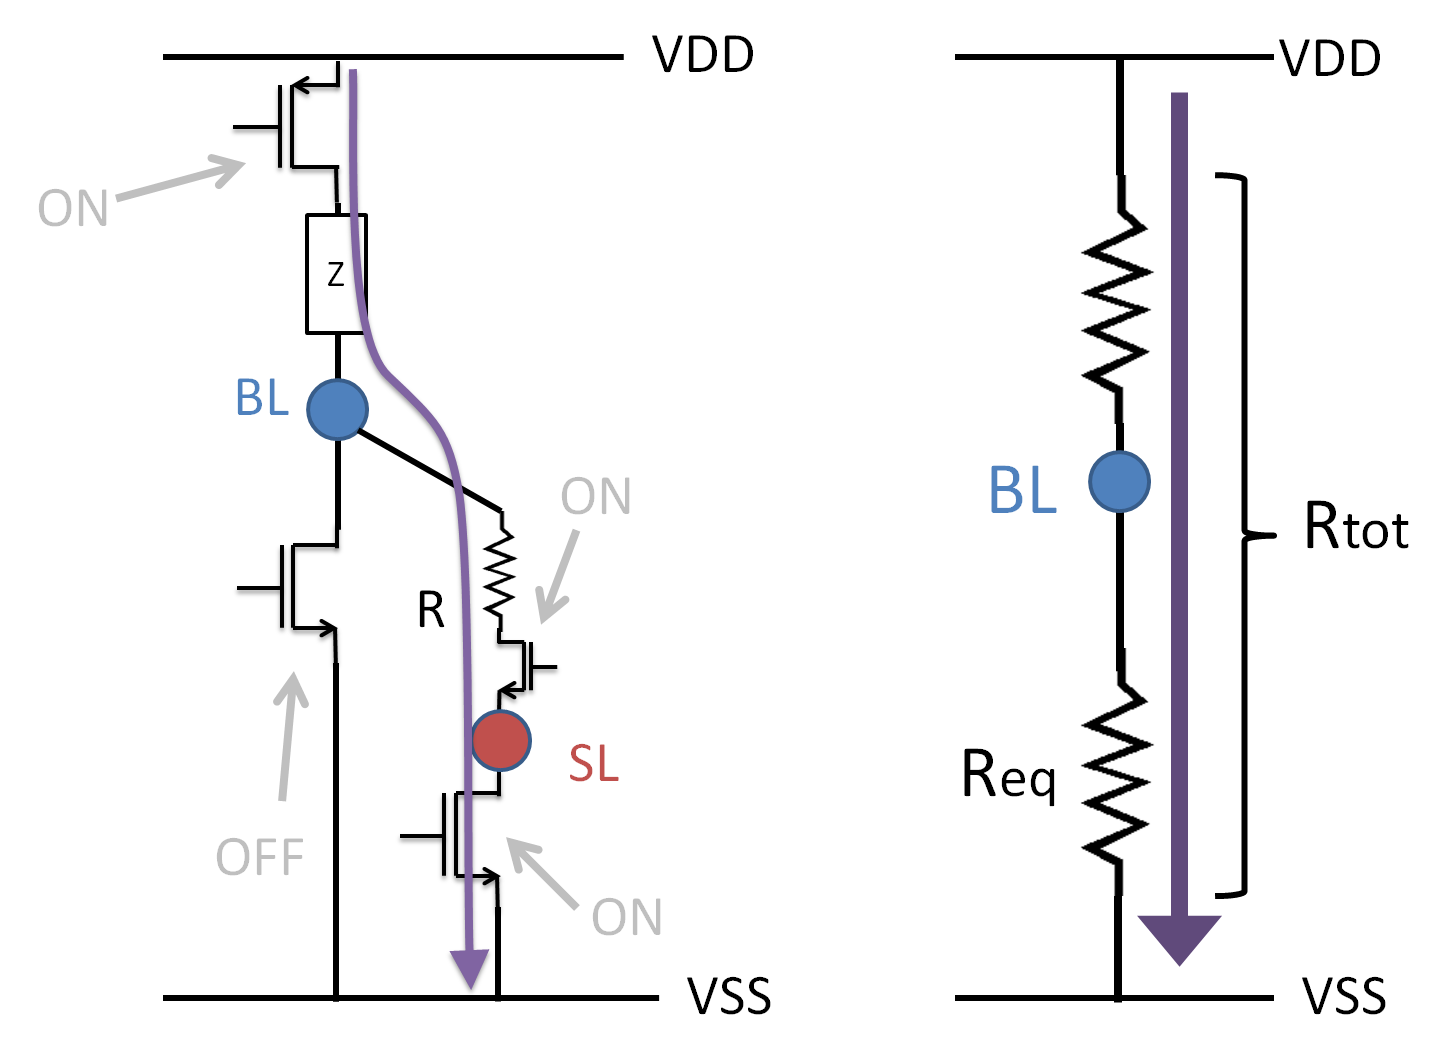
\includegraphics[scale=0.3]{../fig/hfdstk-architecture-datasignal.png}
  \caption{Methodologie om datasignaal te verkrijgen op een BL}
  \label{fig:dataread}
\end{figure}

\subsection{Referentiesignaal uitlezen}
Het referentiesignaal is een spanning die tussen de spanning van een lage resistieve datacel en een hoge resistieve datacel moet liggen. Een dergelijk signaal kan verkregen worden door twee BLs kort te sluiten zoals op figuur \ref{fig:2cellref}. In dit ontwerp zal de kortsluiting gerealiseerd worden door de passgates van de BLs aan te zetten, zo komt het referentiesignaal bovendien ook op de uitgangsknoop te staan. In theorie is het voldoende om 2 BLs [de ene met een HRS cel en de andere met een LRS cel] kort te sluiten om het referentiesignaal te verkrijgen. Er zit echter op de resistieve geheugenelementen variabiliteit: er wordt aangenomen dat $R_{H}$ normaal verdeeld is met $\mu = 32500\Omega$ en $\sigma = 833\Omega$. $R_{L}$ is ook normaal verdeeld met $\mu = 7500\Omega$ en $\sigma = 833\Omega$. Dit betekent dat ook de data-signalen en referentie-signalen stochastische variabelen zijn.
Door echter steeds meer referentiebitlijnen kort te sluiten gaat de spreiding van het referentiesignaal dalen [maar gaat het energieverbruik stijgen]. Bovendien kan men de verwachtingswaarde verschuiven door meer HRS (LRS) referentiegeheugenelementen te gebruiken dan LRS (HRS).

\begin{figure}
  \centering
  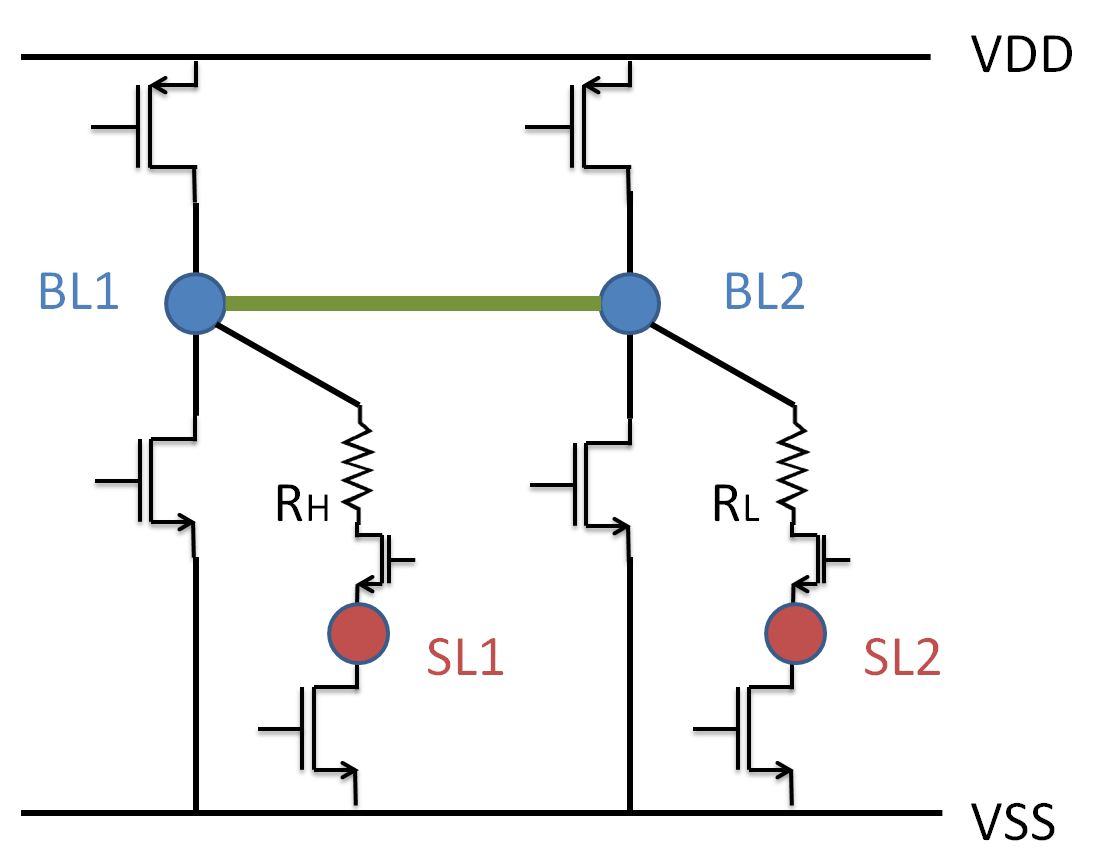
\includegraphics[scale=0.3]{../fig/hfdstk-architecture-ref2cell.png}
  \caption{Topologie om referentiesignaal te verkrijgen}
  \label{fig:2cellref}
\end{figure}

\section{Global Block}
\label{globalblock}
Een global block bestaat uit twee LBs en een sense amplifier (SA) met bijhorende sample-and-hold-schakelaars (S\&H). In het ene LB gaat er een datasignaal geproduceerd worden, in het andere een referentiesignaal (zie figuur \ref{fig:GB}. Vervolgens gaat de SA dit kleine signaalverschil versterken tot een zuivere rail-to-rail output.
Aan de uitgang van het GB verschijnen dan ook de opgevraagde bits.
De laatste architectuurvrijheidsgraad is de \emph{Number of Global Blocks} (NoGB), het totale geheugen bevat dus NoGB x 2 x NoBLpLB x NoWLpB datageheugencellen.

\begin{figure}
  \centering
  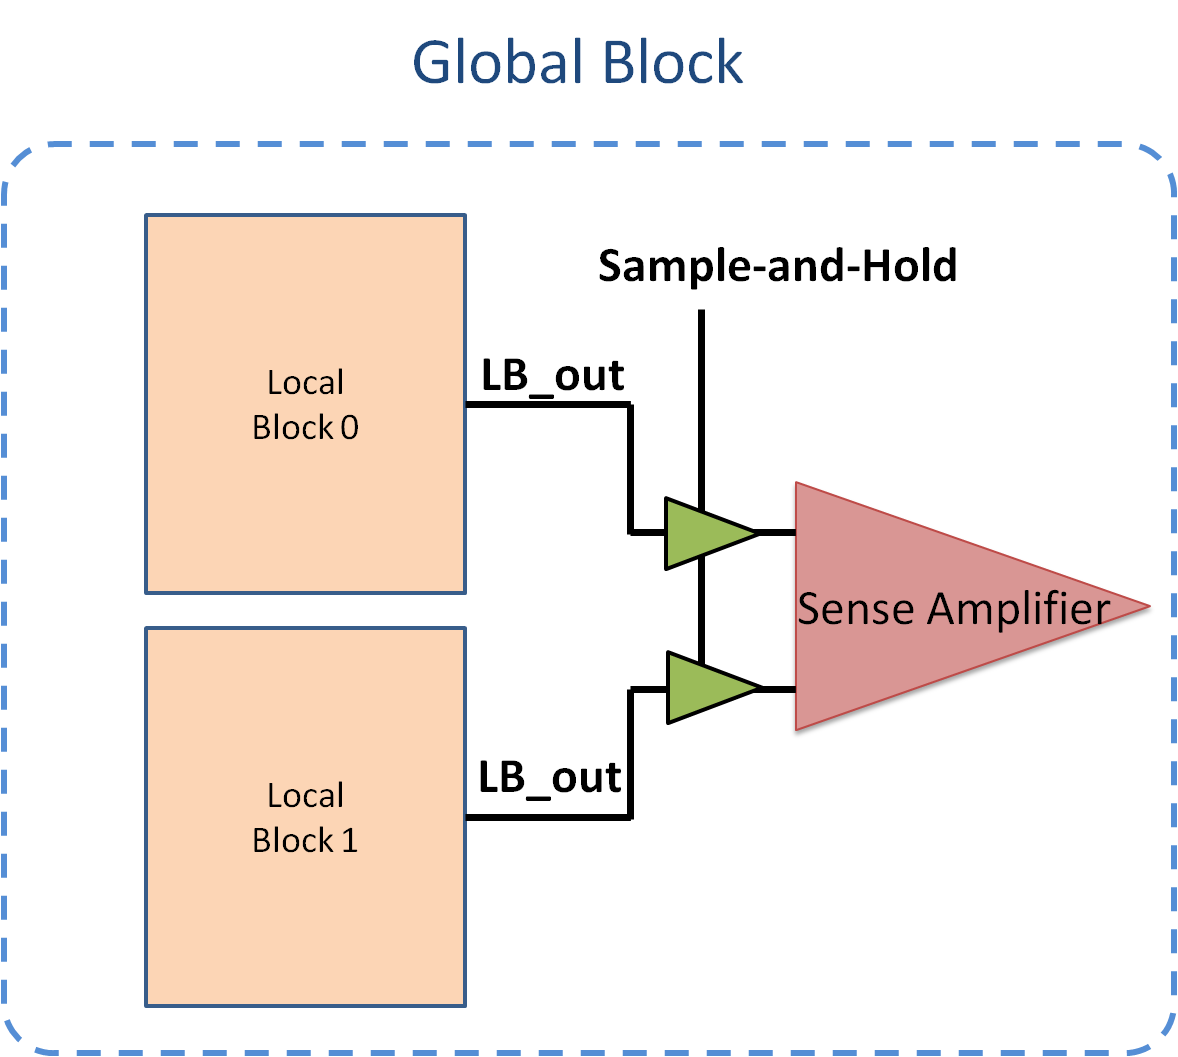
\includegraphics[scale=0.3]{../fig/hfdstk-architecture-globalblock.png}
  \caption{Een Global Block}
  \label{fig:GB}
\end{figure}

\section{Besluit}
De geheugenarchitectuur werd in vogelvlucht overlopen. De kleinste bouwblok is de cel, deze wordt geplaatst in een branch. Verschillende branches vormen samen een local block, dat ook decoders en multiplexers bevat. Twee local blocks en een sense amplifier met bijhorende passgates worden gegroepeerd tot een global block. Het totale geheugen bestaat tenslotte uit een verzameling global blocks.

